%% Created by tikzDevice version 0.5.3 on 2011-02-17 11:33:02
%% Manually edited the colorization, thickness of the lines and cleanup of code on 2011-02-17 12:30
%\documentclass{article}
%\usepackage{tikz}
%
%\usepackage[active,tightpage]{preview}
%
%\PreviewEnvironment{pgfpicture}
%
%\begin{document}
%%%%%%%%%%%%%%%%%%%%%%%%%%%%%%%%%%%%%%%%%
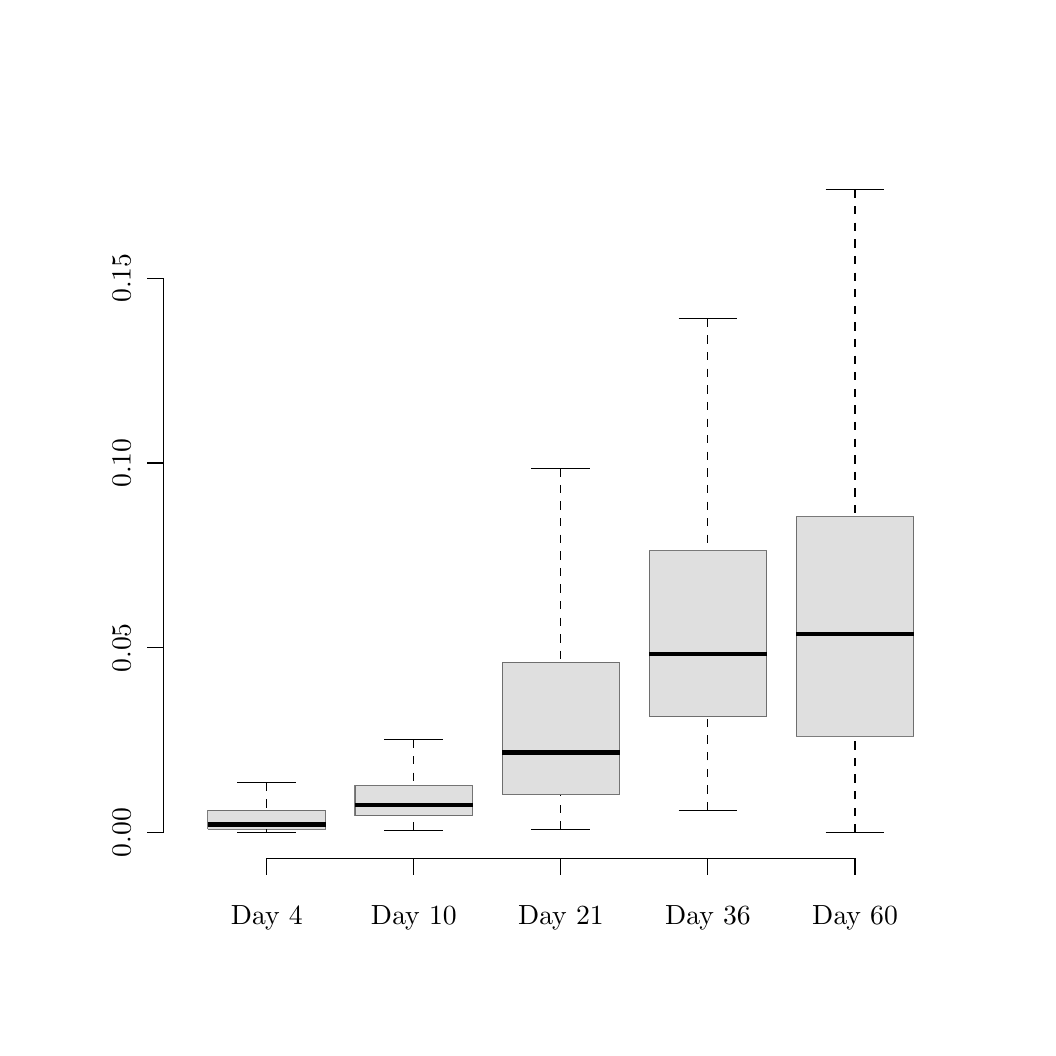
\begin{tikzpicture}[x=1,y=1]
\begin{scope}
%%%%%%%%%%%%%%%%%%%%%D04
\draw[dashed] ( 86.40, 70.52) -- ( 86.40, 71.71);
\draw[dashed] ( 86.40, 88.52) -- ( 86.40, 78.60);
\draw[] ( 75.77, 70.52) -- ( 97.02, 70.52);
\draw[] ( 75.77, 88.52) -- ( 97.02, 88.52);
\draw[fill=lightgray,semitransparent] ( 65.14, 71.71) --
	(107.65, 71.71) --
	(107.65, 78.60) --
	( 65.14, 78.60) --
	( 65.14, 71.71);
\draw[ultra thick] ( 65.14, 73.35) -- (107.65, 73.35);	
%%%%%%%%%%%%%%%%%%%%%D10
\draw[dashed] (139.54, 71.17) -- (139.54, 76.51);
\draw[dashed] (139.54,104.14) -- (139.54, 87.58);
\draw[] (128.91, 71.17) -- (150.16, 71.17);
\draw[] (128.91,104.14) -- (150.16,104.14);
\draw[fill=lightgray,semitransparent] (118.28, 76.51) --
	(160.79, 76.51) --
	(160.79, 87.58) --
	(118.28, 87.58) --
	(118.28, 76.51);
\draw[ultra thick] (118.28, 80.53) -- (160.79, 80.53);
%%%%%%%%%%%%%%%%%%%%%D21
\draw[dashed] (192.67, 71.64) -- (192.67, 84.24);
\draw[dashed] (192.67,202.16) -- (192.67,132.05);
\draw[] (182.05, 71.64) -- (203.30, 71.64);
\draw[] (182.05,202.16) -- (203.30,202.16);
\draw[fill=lightgray,semitransparent] (171.42, 84.24) --
	(213.93, 84.24) --
	(213.93,132.05) --
	(171.42,132.05) --
	(171.42, 84.24);
\draw[ultra thick] (171.42, 99.47) -- (213.93, 99.47);
%%%%%%%%%%%%%%%%%%%%%D36
\draw[dashed] (245.81, 78.61) -- (245.81,112.29);
\draw[dashed] (245.81,256.12) -- (245.81,172.38);
\draw[] (235.19, 78.61) -- (256.44, 78.61);
\draw[] (235.19,256.12) -- (256.44,256.12);
\draw[fill=lightgray,semitransparent] (224.56,112.29) --
	(267.07,112.29) --
	(267.07,172.38) --
	(224.56,172.38) --
	(224.56,112.29);
\draw[ultra thick] (224.56,134.99) -- (267.07,134.99);
%%%%%%%%%%%%%%%%%%%%%D60
\draw[dashed] (298.95, 70.49) -- (298.95,105.34);
\draw[dashed] (298.95,302.86) -- (298.95,184.67);
\draw[] (288.32, 70.49) -- (309.58, 70.49);
\draw[] (288.32,302.86) -- (309.58,302.86);
\draw[fill=lightgray,semitransparent] (277.70,105.34) --
	(320.21,105.34) --
	(320.21,184.67) --
	(277.70,184.67) --
	(277.70,105.34);
\draw[ultra thick] (277.70,142.20) -- (320.21,142.20);	
\end{scope}
\begin{scope}
\path[clip] (  0.00,  0.00) rectangle (361.35,361.35);

\draw[] ( 86.40, 61.20) -- (298.95, 61.20);
\draw[] ( 86.40, 61.20) -- ( 86.40, 55.20);
\draw[] (139.54, 61.20) -- (139.54, 55.20);
\draw[] (192.67, 61.20) -- (192.67, 55.20);
\draw[] (245.81, 61.20) -- (245.81, 55.20);
\draw[] (298.95, 61.20) -- (298.95, 55.20);

\node[anchor=base,] at ( 86.40, 37.20) {Day 4};
\node[anchor=base,] at (139.54, 37.20) {Day 10};
\node[anchor=base,] at (192.67, 37.20) {Day 21};
\node[anchor=base,] at (245.81, 37.20) {Day 36};
\node[anchor=base,] at (298.95, 37.20) {Day 60};

\draw[] ( 49.20, 70.49) -- ( 49.20,270.81);
\draw[] ( 49.20, 70.49) -- ( 43.20, 70.49);
\draw[] ( 49.20,137.26) -- ( 43.20,137.26);
\draw[] ( 49.20,204.03) -- ( 43.20,204.03);
\draw[] ( 49.20,270.81) -- ( 43.20,270.81);

\node[rotate= 90.00,anchor=base,] at ( 37.20, 70.49) {0.00};
\node[rotate= 90.00,anchor=base,] at ( 37.20,137.26) {0.05};
\node[rotate= 90.00,anchor=base,] at ( 37.20,204.03) {0.10};
\node[rotate= 90.00,anchor=base,] at ( 37.20,270.81) {0.15};

%\draw[] ( 49.20, 61.20) --
%	(336.15, 61.20) --
%	(336.15,312.15) --
%	( 49.20,312.15) --
%	( 49.20, 61.20);
\end{scope}
\end{tikzpicture}
%%%%%%%%%%%%%%%%%%%%%%%%%%%%%%%%%%%%%%%%%
%\end{document}